\documentclass[onecolumn,nofootinbib,superscriptaddress]{revtex4}

\usepackage{multirow, makecell}
\usepackage{amsfonts}
\usepackage{amsmath}
\usepackage{amssymb}
\usepackage{bm}
\usepackage{dcolumn}
\usepackage{epsfig}
\usepackage{graphicx}
\usepackage{graphics}
\usepackage[latin1]{inputenc}
\usepackage{latexsym}
\usepackage{rotating}
\usepackage[colorlinks=true]{hyperref}
\usepackage[usenames]{color}
\usepackage{yfonts}
\usepackage{float}
\usepackage{ucs}
\usepackage{xspace} % Sensible space treatment at end of simple macros
\usepackage{mathrsfs}
\usepackage{subfig}
\usepackage{enumitem}
\usepackage{tabularx}
\usepackage{booktabs}
\usepackage{siunitx}
\usepackage{array}
\usepackage[normalem]{ulem}
\usepackage[english]{babel}

\newcommand{\dd}[1]{\mathrm{d}#1\,}

\newcommand{\rs}[1]{\textcolor{blue}{\it{\textbf{RS: #1}}} }
\newcommand{\stst}[1]{\textcolor{blue}{\it{\textbf{SS: #1}}} }


\begin{document}

\title{Gravitational Radiation from Quantum Turbulence in Superfluid Dark Matter Halos}

\author{R.C. Greene}
\affiliation{Columbia?}
\author{Robert Sims}
\email{robert\_sims@brown.edu}
\affiliation{Department of Physics, Brown University, Providence, RI, 02906}
\author{Stefan Stanojevic}
\affiliation{Department of Physics, Brown University, Providence, RI, 02906}


\begin{abstract}
.
\end{abstract}


\date{\today}

\maketitle


\section{Superfluids and Quantum Turbulence}

Consider the Lagrangian for a complex scalar field theory with quartic self-interactions:
\begin{equation}
\mathcal{L} = -|\partial_\mu \phi|^2 - m^2|\phi|^2 - \frac{\lambda}{2}|\phi|^4.
\end{equation}
We work in the weak-field regime, $g_{\mu\nu} = \eta_{\mu\nu} -2\Phi I_{\mu\nu}$, where $\eta_{\mu\nu}$ is the Minkowski metric, $I_{\mu\nu}$ is the identity matrix, and $\Phi$ is the gravitational potential.  When working in the non-relativistic regime, we can explicitly write the highly oscillating behavior of $\phi$ as
\begin{equation}
\phi({\bf{x}},t) = \frac{1}{\sqrt{2m}}\psi({\bf{x}},t)e^{-imt},
\end{equation}
where $\psi$ is a slowly varying function in time.  {\rs{See \cite{Chavanis:2016shp} for the inclusion of interactions with electromagnetism. This reference is very good for going through all of basic equations in the theory, specifically after decomposing the scalar into amplitude and phase.}} The equation of motion for the complex scalar $\psi$ can be approximated by the Schr\"{o}dinger-Poisson equation.  In terms of dimensionless quantities,
\begin{gather}
i\Psi' = -\frac{1}{2}\tilde{\nabla}^2\Psi + \Phi\Psi + \tilde{\lambda}|\Psi|^2\Psi,\label{EQ:ScalarEoM}\\
\tilde{\nabla}^2\Phi = |\Psi|^2,
\end{gather}
where the $'$ denotes derivatives with respect to the dimensionless time variable $m t$, and $\Psi = \sqrt{m}\psi/\sqrt{4\pi G}, \tilde{\nabla} = \nabla /m, \tilde{\lambda} = \lambda/16\pi G m^2$. {\rs{There are two ways to make these equations dimensionless.  Other than what is written here, we can write lengths/distances in terms of $G$, i.e. in Planck units.  Using Planck units may be more useful for simulating the entire halo, but I think these units may be more useful for the simulation of a small cluster of vortices.}}

\stst{Simulation uses different 'natural units' so this part can change. Equations (1), (3) are missing gravity}

The scalar field equations of motion can be rewritten as fluid equations by the Madelung transformation:
\begin{equation}
\label{eq:defrhov}
\Psi = \sqrt{\rho}\exp(i\theta), \;\;\;\;\;\; {\bf{u}} = \tilde{\nabla}\theta,
\end{equation}
where $\rho, \theta$ are real functions, and ${\bf{u}}$ is the flow velocity.  Decomposing Eq.~(\ref{EQ:ScalarEoM}) into real and imaginary parts, the system is described in fluid variables by
\begin{gather}
\tilde{\nabla}^2\Phi = \rho,\\
\rho' + \tilde{\nabla}\cdot(\rho {\bf{u}}) = 0,\\
{\bf{u}}' + \frac{1}{2}\tilde{\nabla}(u^2) = -\tilde{\nabla}\left(\Phi + \tilde{\lambda}\rho - \frac{\tilde{\nabla}^2\rho}{4\rho}+\frac{(\tilde{\nabla}\rho)^2}{8\rho^2}\right).
\end{gather}
We note, the quartic self-interaction of the boson manifests as a source term in the velocity equation of motion.  This term is distinct from a viscosity, since there is no explicit dependence on velocity.  Instead, depending on the sign of $\lambda$, the fluid will flow to either fill or evacuate underdense regions.

Madelung transformation allows us to apply standard theory of fluid dynamics to a BEC. One notable difference between a superfluid and conventional fluid is that velocity field, defined as in (\ref{eq:defrhov}) is necessarily curl-free. From the Stokes theorem, such a field will have zero circulation around an arbitrary contour so long as the field is analytic at every point inside the contour. As a consequence, superfluids will carry angular momentum only when vortices, at the center of which velocity field blows up and density decays to zero, are present. The amount of angular momentum carried by vortices will be quantized. 

\stst{Will add the functional form of density and velocity for isolated vortices here. Also, angular momentum of vortices and healing length. Comment on how the healing length in purely  self-gravitational case may be many orders of magnitude different?}

While turbulence in conventional fluids is driven by presence of and interactions between edies, turbulence in superfluids occurs due to interactions of vortices. In order to study this process mathematically, one customarily starts by Helmholtz decomposition of \textit{density weighted velocity} field, $v = \sqrt{\rho} u$ into a divergence-free and curl-free parts, denoted by $v^{(i)}$ and $v^{(c)}$ respectively. The former, 'compressible' part, captures the motion of mechanical waves in the system, while the latter, 'incompressible' component is responsible for turbulence. 

Turbulence is characterized by an \textit{energy cascade} from large to small scales, captured using the \textit{velocity correlation tensor} defined as

\begin{align}
R_{a b}(r) = \langle v^{(i)}_a(r' + r) v^{(i)}_b(r') \rangle_{r'}
\end{align}
 
The Fourier transform of $R_{a b}(r)$ will be denoted as $\tilde{R}_{a b}(k)$. Then, the energy spectrum is defined as

\begin{align}
E(k) = 2 \pi k^2 \sum_i \tilde{R}_{i i}(k) 
\end{align}

Turbulence is diagonosed by the power law decay of the energy spectrum. Conventional fluids typically feature the Kolmogorov spectrum, $E(k) \propto k^{-5/3}$, while superfluids studied in a laboratory feature different power laws with exponents greater or equal to $-5/3$, depending on how turbulence is induced.

\stst{References need to be added all over the place... Also, need to comment on dissipation in two-component superfluid and Kelvin waves}


\section{Simulations}

We used the approach of \cite{Mocz:2017wlg} to numerically solve the field equations, featuring periodic boundary conditions and a pseudospectral symplectic method. Fast fourier transform routine is used to solve for the gravitational potential at each time step, during which the field is time evolved separately with respect to potential and kinetic parts of the Hamiltonian, in a leapfrog-like manner. 


In the case of zero angular momentum, the simulation reproduces the known solutions 
{\stst{Which we should include and cite \cite{Schiappacasse:2017ham}. Also, perhaps cite \cite{Hertzberg:2018lmt} and simulate the symmetric case with non-zero angular momentum}

We were interesting in the effect of infusing a stable zero-momentum halo configuration with vortices. The results are shown in Fig (\ref{fig:sub2}). 

\begin{figure}[ht]  
\label{fig:1}
\centering    
\subfloat[Density]{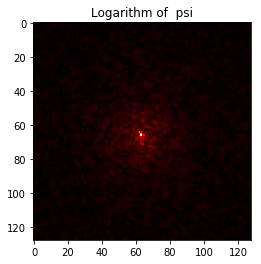
\includegraphics[width=0.3\textwidth, keepaspectratio]{Sample_density.png}\label{fig:subfig5}}    
\subfloat[Phase]{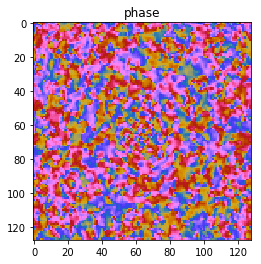
\includegraphics[width=0.3\textwidth, keepaspectratio]{Sample_phase.png}\label{fig:subfig6}}    
\caption{placeholder}    
\label{fig:sub2}
\end{figure}

\begin{figure}
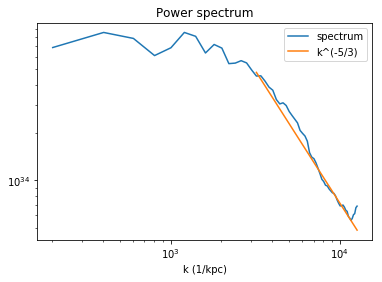
\includegraphics[width=0.5\textwidth, keepaspectratio]{spectrum.png}
\end{figure}

\section{Gravitational Waves from Turbulent Fluid}

Tensor mode perturbations of the metric are sourced by the transverse and traceless component of the anisotropic stress-energy tensor, $\Pi_{ij}$. Assuming there are negligible gravitational waves before the source is turned on, Green's functions methods give the gravitational wave solution
\begin{equation}
h_{ij}({\bf{k}},t) = 8\pi G\int G_k(t,t')\Pi_{ij}({\bf{k}},t') dt',
\end{equation}
where $G_k(t,t')$ is the retarded Green's function.  We will be interested in gravitational radiation produced in a gravitational bound system.  Thus, the retarded Green's function can be found  as {\rs{We should make sure the effects of gravitational lensing should not be included here.  Also, this Green's function may change, depending on the specific details of situtaion, i.e. before halo formation, during the formation of a halo, or after stable halo configuration.  Right now, I think we should focus on stable halos, so this is the most relevant form.}}
\begin{equation}
G_k(t,t') = \frac{1}{k}\sin\left(k(t-t')\right)\Theta(t-t'),
\end{equation}
where the Heaviside step function $\Theta(t-t')$ will impose causality.

For a turbulent fluid with a spatial velocity distribution $\bf{u}(\bf{x})$, the Fourier space stress tensor is given \cite{Kosowsky:2001xp} by
\begin{equation}
\Pi_{ij}({\bf{k}},t) = \left(P_{il}(\hat{\bf{k}})P_{jm}(\hat{\bf{k}})-\frac{1}{2}P_{ij}(\hat{\bf{k}})P_{lm}(\hat{\bf{k}})\right)\frac{\omega V}{(2\pi)^3}\int d{\bf{q}} \,u_l({\bf{q}},t)u_m({\bf{k}}-{\bf{q}},t),
\end{equation}
where $P_{ij}(\hat{\bf{k}})$ is the projection operator onto the transverse plane of ${\bf{k}}$, $V$ is a volume included for dimensional reasons, and $\omega$ is the enthalpy density, equal to the sum of energy density and pressure of the nonturbulent fluid.









\begin{thebibliography}{99}

%\cite{Chavanis:2016shp}
\bibitem{Chavanis:2016shp} 
  P.~H.~Chavanis and T.~Matos,
  \emph{Covariant theory of Bose-Einstein condensates in curved spacetimes with electromagnetic interactions: the hydrodynamic approach},
  Eur.\ Phys.\ J.\ Plus {\bf 132}, no. 1, 30 (2017)
  %doi:10.1140/epjp/i2017-11292-4
  [arXiv:1606.07041 [gr-qc]].
  %%CITATION = doi:10.1140/epjp/i2017-11292-4;%%
  %8 citations counted in INSPIRE as of 02 Mar 2018

%\cite{Fan:2016rda}
\bibitem{Fan:2016rda} 
  J.~Fan,
  \emph{Ultralight Repulsive Dark Matter and BEC},
  Phys.\ Dark Univ.\  {\bf 14}, 84 (2016)
  %doi:10.1016/j.dark.2016.10.005
  [arXiv:1603.06580 [hep-ph]].
  %%CITATION = doi:10.1016/j.dark.2016.10.005;%%
  %15 citations counted in INSPIRE as of 02 Mar 2018

%\cite{Kosowsky:2001xp}
\bibitem{Kosowsky:2001xp} 
  A.~Kosowsky, A.~Mack and T.~Kahniashvili,
  \emph{Gravitational radiation from cosmological turbulence},
  Phys.\ Rev.\ D {\bf 66}, 024030 (2002)
  %doi:10.1103/PhysRevD.66.024030
  [astro-ph/0111483].
  %%CITATION = doi:10.1103/PhysRevD.66.024030;%%
  %139 citations counted in INSPIRE as of 27 Feb 2018
  
  %\cite{Mocz:2017wlg}
\bibitem{Mocz:2017wlg} 
  P.~Mocz, M.~Vogelsberger, V.~H.~Robles, J.~Zavala, M.~Boylan-Kolchin, A.~Fialkov and L.~Hernquist,
  %``Galaxy formation with BECDM – I. Turbulence and relaxation of idealized haloes,''
  Mon.\ Not.\ Roy.\ Astron.\ Soc.\  {\bf 471}, no. 4, 4559 (2017)
  doi:10.1093/mnras/stx1887
  [arXiv:1705.05845 [astro-ph.CO]].
  %%CITATION = doi:10.1093/mnras/stx1887;%%
  %11 citations counted in INSPIRE as of 26 Apr 2018

%\cite{Schiappacasse:2017ham}
\bibitem{Schiappacasse:2017ham} 
  E.~D.~Schiappacasse and M.~P.~Hertzberg,
  %``Analysis of Dark Matter Axion Clumps with Spherical Symmetry,''
  JCAP {\bf 1801}, 037 (2018)
  Erratum: [JCAP {\bf 1803}, no. 03, E01 (2018)]
  doi:10.1088/1475-7516/2018/03/E01, 10.1088/1475-7516/2018/01/037
  [arXiv:1710.04729 [hep-ph]].
  %%CITATION = doi:10.1088/1475-7516/2018/03/E01, 10.1088/1475-7516/2018/01/037;%%
  %6 citations counted in INSPIRE as of 26 Apr 2018}
  
  %\cite{Hertzberg:2018lmt}
\bibitem{Hertzberg:2018lmt} 
  M.~P.~Hertzberg and E.~D.~Schiappacasse,
  %``Scalar Dark Matter Clumps with Angular Momentum,''
  arXiv:1804.07255 [hep-ph].
  %%CITATION = ARXIV:1804.07255;%%

\end{thebibliography}

\end{document}